\frame
{
\frametitle{Venta de la licencia de su tecnología más avanzada}
\begin{table}
\begin{tabular}{p{7cm}p{3cm}}
\begin{itemize}
    \item Vender ideas en cuanto son comercializables.
    \item Imponerse a propósito más presión sobre sí mismo.
\end{itemize}
&
\vspace{1.5cm}
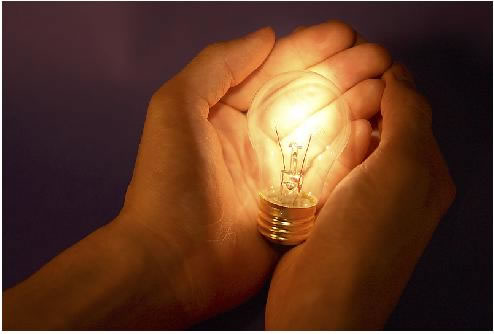
\includegraphics[width=4cm]{img/innovar.jpg}\\
\end{tabular}
\end{table}
}

\frame
{
\frametitle{Canibalice sus productos más rentables}
\begin{table}
\begin{tabular}{p{7cm}p{3cm}}
\begin{itemize}
    \item Lanzar nuevos productos sin importar que compitan con los viejos
    productos de la empresa.
\end{itemize}
&
\vspace{1.5cm}
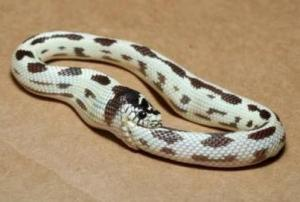
\includegraphics[width=4cm]{img/ouroboros.jpg}\\
\end{tabular}
\end{table}
}
\frame
{
\frametitle{Venda/divida nuevas unidades}
\begin{table}
\begin{tabular}{p{7cm}p{3cm}}
\begin{itemize}
    \item Cultura organizacional no permite diferentes enfoques.
    \item Equipos paralelos de trabajo.
\end{itemize}
&
\vspace{1.5cm}
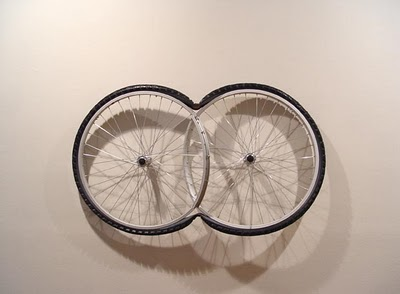
\includegraphics[width=4cm]{img/mitosis.jpg}\\
\end{tabular}
\end{table}
}
\frame
{
\frametitle{Liquide los viejos éxitos para forzar la dependencia de los nuevos}
\begin{table}
\begin{tabular}{p{7cm}p{3cm}}
\begin{itemize}
    \item \textit{Deshacerse} de uno o más productos muy rentables, mientras
    todavía sean rentables.
    \item Obliga a depender de las líneas más nuevas del negocio.
\end{itemize}
&
\vspace{1.5cm}

\includegraphics[width=4cm]{img/getting_older.jpg}\\
\end{tabular}
\end{table}
}
\frame
{
\frametitle{Financie la audacia}
\begin{table}
\begin{tabular}{p{7cm}p{3cm}}
\begin{itemize}
    \item Financiar a las \textit{mentes brillantes} de la propia empresa.
    \item Evita que éstas abandonen la empresa, o caigan sofocados bajo
    prejuicios.
    \item Ser un \textit{Capitalista de Riesgo}.
\end{itemize}
&
\vspace{1.5cm}

\includegraphics[width=4cm]{img/creativegenius.jpg}\\
\end{tabular}
\end{table}
}
\frame
{
\frametitle{Vender cuota sustancial de los productos o servicios al mercado
exterior}
\begin{table}
\begin{tabular}{p{7cm}p{3cm}}
\begin{itemize}
    \item Demostrar aptitud para competir.
    \item Cada unidad de la empresa debe estar involucrado.
    \item Competir contra los mejores.
\end{itemize}
&
\vspace{1.5cm}

\includegraphics[width=4cm]{img/openbusiness.jpg}\\
\end{tabular}
\end{table}
}
\frame
{
\frametitle{Forzar la competencia entre las funciones internas con las
externas.}
\begin{table}
\begin{tabular}{p{7cm}p{3cm}}
\begin{itemize}
    \item Estimular que las unidades cercanas al mercado compren los mejores
    productos y servicios, incluyendo a los de la competencia.
\end{itemize}
&
\vspace{1.5cm}
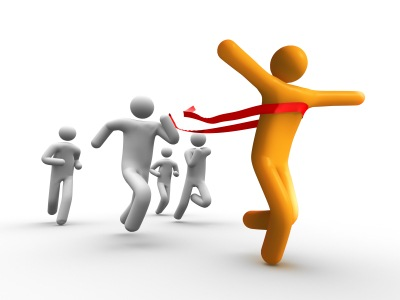
\includegraphics[width=4cm]{img/competition.jpg}\\
\end{tabular}
\end{table}
}
\frame
{
\frametitle{Subcontrate absolutamente todo}
\begin{table}
\begin{tabular}{p{7cm}p{3cm}}
\begin{itemize}
    \item Subcontratación como forma de vida.
    \item Red de subcontratistas.
    \item La innovación es lo importante.
\end{itemize}
&
\vspace{1.5cm}
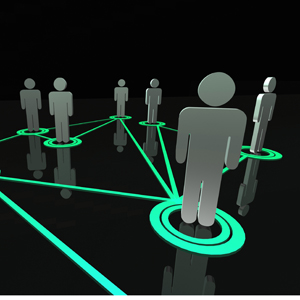
\includegraphics[width=4cm]{img/subcontract.jpg}\\
\end{tabular}
\end{table}
}
\frame
{
\frametitle{Crear numerosas joint-ventures y alianzas}
\begin{table}
\begin{tabular}{p{7cm}p{3cm}}
\begin{itemize}
    \item Trabaje con todo el mundo, de cualquier parte, durante un periodo
    corto o largo.
    \item Especialmente con empresas nuevas y del exterior.
\end{itemize}
&
\vspace{1.5cm}
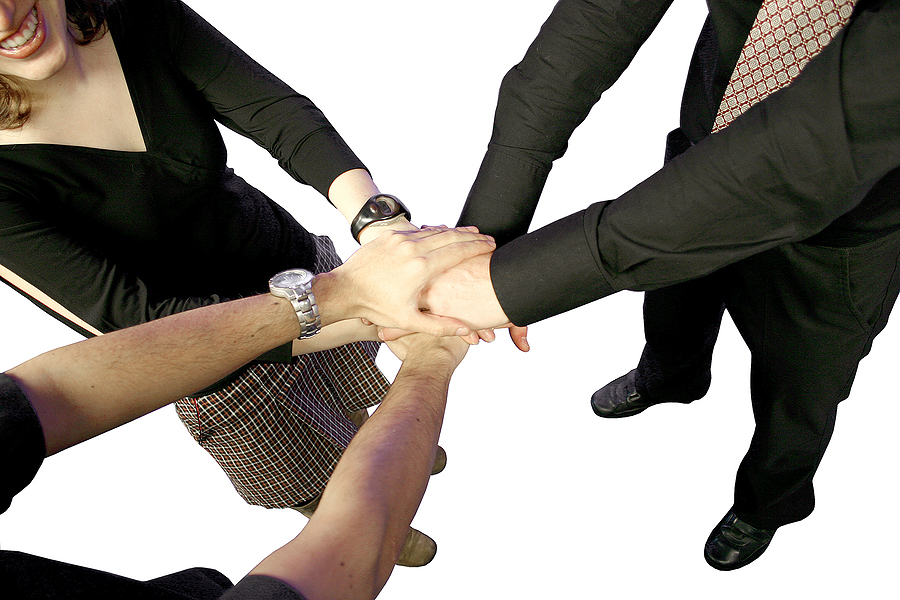
\includegraphics[width=4cm]{img/joint-venture.jpg}\\
\end{tabular}
\end{table}
}
